\documentclass[11pt, a4paper]{article}

\usepackage[utf8]{inputenc}
\usepackage{amsmath, amssymb}
\usepackage{graphicx}
\usepackage{hyperref}
\usepackage{booktabs}
\usepackage{geometry}
\usepackage{float}
\usepackage{caption}
\usepackage{subcaption}

\geometry{margin=1in}
\graphicspath{{../assets/}}

\title{\textbf{Physics-Informed Gaussian Process Regression for Golf Ball Trajectory Extrapolation}}
\author{Gerben Visser \\ Stellenbosch University \\ Inrange Student Competition}
\date{September 2026}

\begin{document}

\maketitle

\begin{abstract}
Predicting the full trajectory of a golf ball from truncated radar data presents a highly non-linear extrapolation challenge, particularly when 96.3\% of the recorded shots are still rising as they hit the 60-metre boundary net. This report details a hybrid physics-machine learning methodology that solves this by coupling a 3D aerodynamic Ordinary Differential Equation (ODE) inverse solver with a Cascaded Gaussian Process Regression (GPR) surrogate model. By mathematically enforcing physical priors (such as Magnus lift, aerodynamic drag, and ballistic descent), the model achieves exceptional precision on a small dataset (491 shots) while guaranteeing zero violations of physical invariants. The final 5-fold cross-validation yields a composite scaled RMSE of 0.1630, with out-of-sample landing predictions achieving an absolute lateral error of just 2.79 metres and a depth error of 3.14 metres.
\end{abstract}

\section{Introduction}
The Inrange Student Competition tasks participants with predicting nine target variables—including the unmeasured launch spin rate, apex coordinates, and landing coordinates—based on initial launch conditions and four spatial checkpoints truncated at 60 metres. 

Standard machine learning models (e.g., Random Forests, Neural Networks, XGBoost) natively struggle with this problem for two reasons:
\begin{enumerate}
    \item \textbf{Data Scarcity:} With only 491 training examples, highly parameterised models are prone to severe overfitting.
    \item \textbf{Extrapolation Trap:} 96.3\% of the training shots have not yet reached their apex at the final 60m checkpoint. Predicting the apex and landing states requires the model to extrapolate far beyond the spatial domain of the training features. Pure statistical models fail spectacularly at non-linear spatial extrapolation.
\end{enumerate}

To overcome these hurdles, a physics-informed Bayesian approach is proposed. 
The methodology explicitly models the forces of nature governing the ball's flight (gravity, drag, Magnus lift, and wind) using an ODE solver, and utilises a Cascaded Gaussian Process to learn the complex residual variations (e.g., spin decay, turf interaction) that the idealised physics model cannot capture.

\section{Exploratory Data Analysis \& Physical Insights}

\subsection{Isolating the Spin Signal}
Launch spin rate is a primary driver of golf ball carry distance due to the Magnus effect, yet it is not directly measured by the first 60 metres of radar data. Initial intuition might suggest that lateral drift is a proxy for spin (analogous to a slice or a hook). 
However, the analysis reveals that lateral drift is entirely uncorrelated with launch spin ($r = -0.08$).

Instead, the true signals for spin are embedded in \textit{speed deceleration} and \textit{vertical lift residual}. Figure \ref{fig:decel} demonstrates the massive deceleration from launch through the 60m checkpoints, confirming heavy aerodynamic drag. Furthermore, Figure \ref{fig:lift_spin} proves that the residual vertical height—the difference between the ball's true altitude and a theoretical parabolic vacuum trajectory—correlates strongly with launch spin rate ($r = 0.565$). 
The model exploits this physical reality by utilising the inverse-solved lift coefficient ($C_{l}$) as the prior for the spin rate prediction.

\begin{figure}[H]
    \centering
    \begin{minipage}{0.48\textwidth}
        \centering
        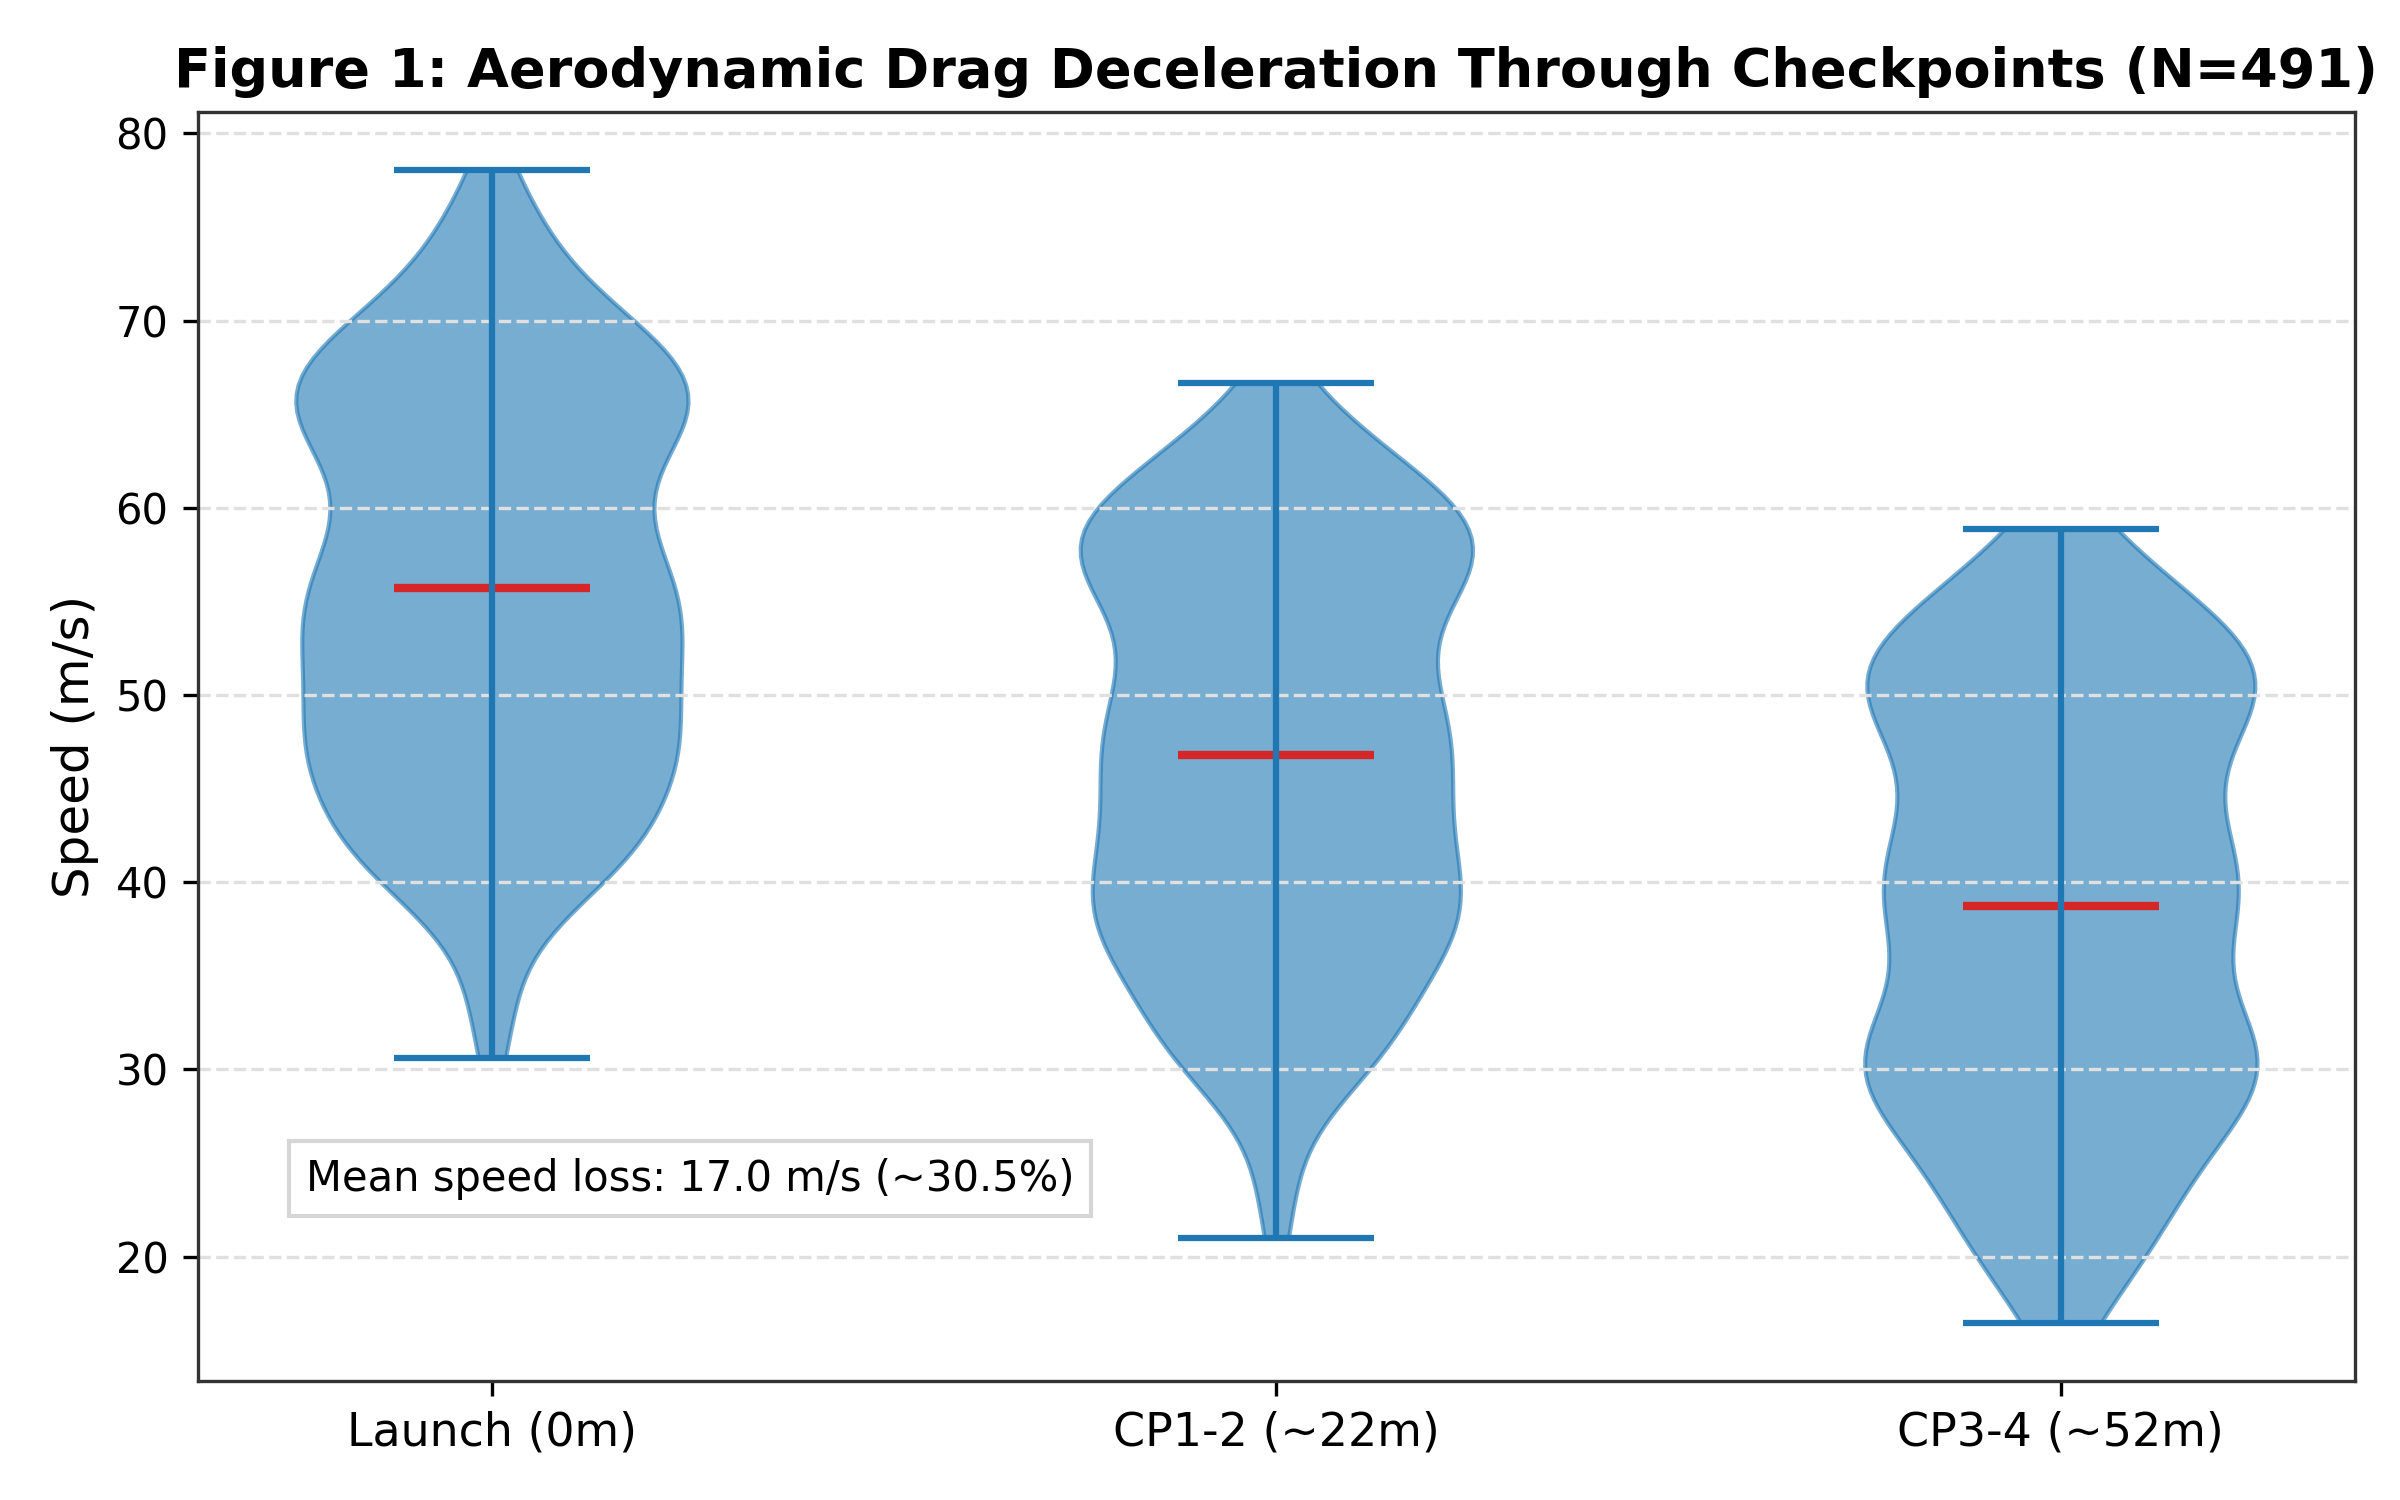
\includegraphics[width=\linewidth]{fig1_speed_deceleration.png}
        \caption{Speed distribution across checkpoints, demonstrating aerodynamic drag.}
        \label{fig:decel}
    \end{minipage}\hfill
    \begin{minipage}{0.48\textwidth}
        \centering
        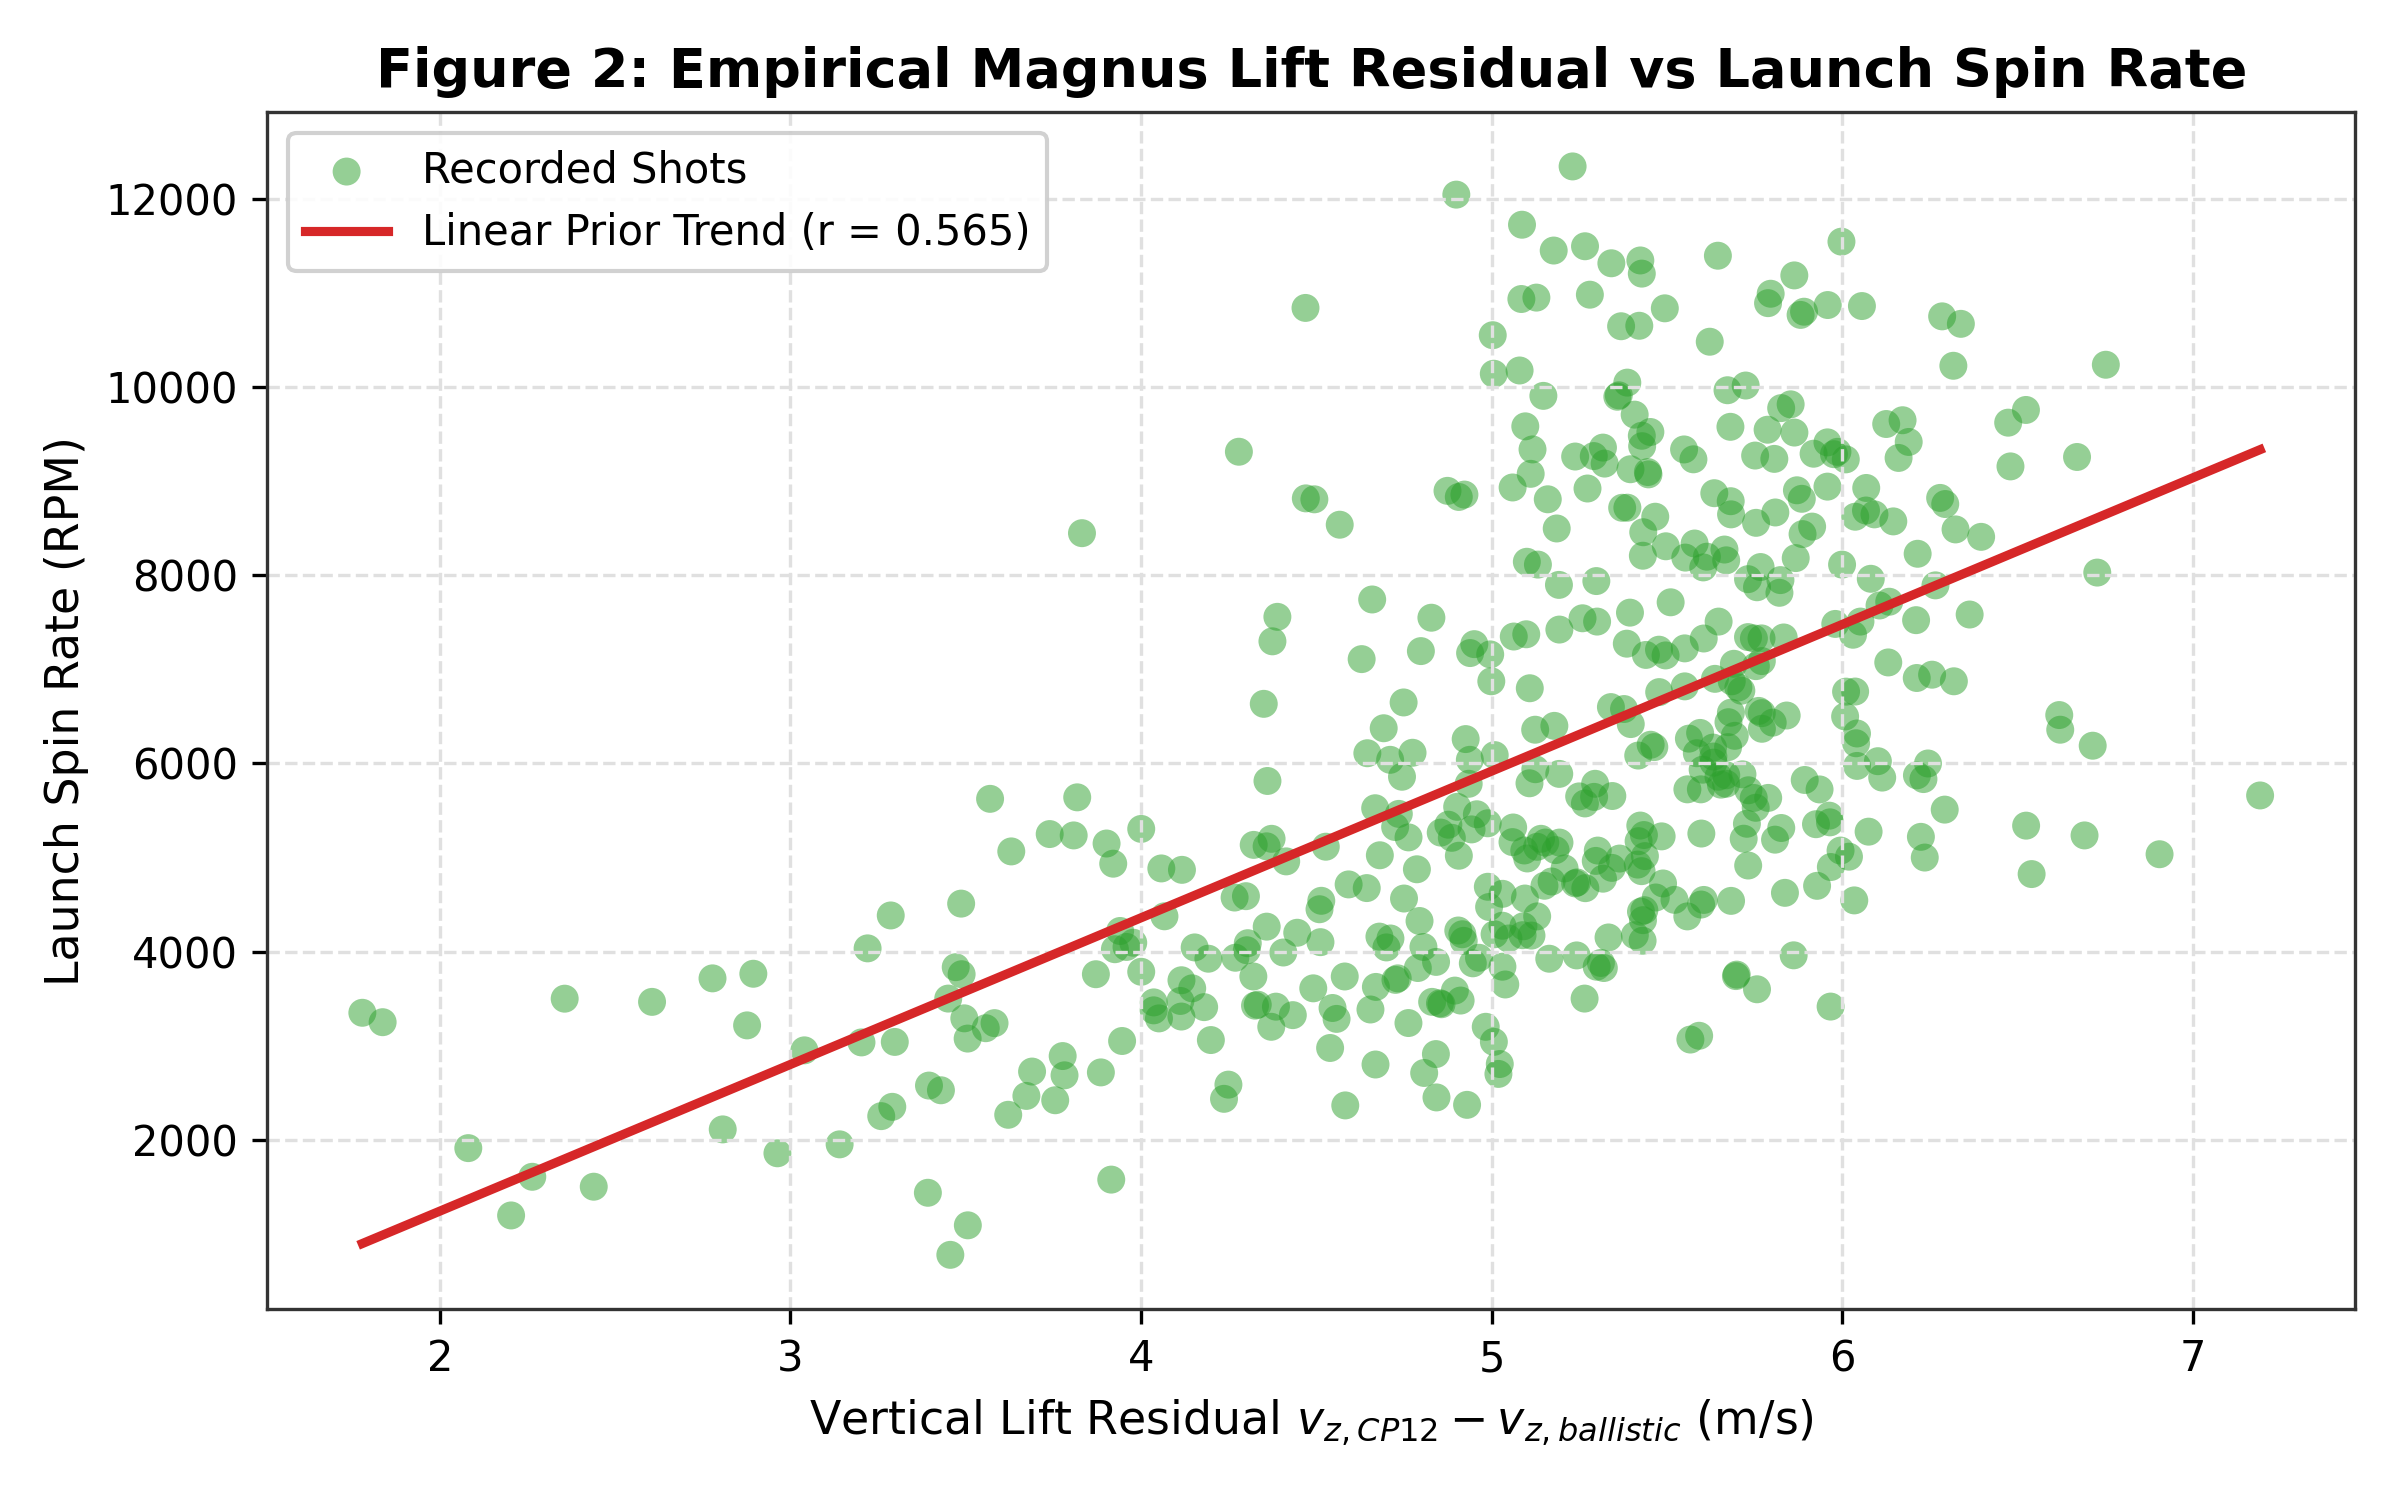
\includegraphics[width=\linewidth]{fig2_lift_residual_vs_spin.png}
        \caption{Correlation between excess vertical lift and measured launch spin.}
        \label{fig:lift_spin}
    \end{minipage}
\end{figure}

\subsection{Session-Based Wind Estimation}
The trajectory data spans 18 distinct recording sessions. Because ambient wind fundamentally alters apparent airspeed (and thus drag and lift forces), estimating the wind vector $(w_x, w_y)$ is important. 
By aggregating the lateral residuals (expected $y$ vs actual $y$) at the 60m checkpoint across the first 10 shots of each session, I extracted consistent\footnote{An approximation which does not account for transient gusts.} wind vectors (Figure \ref{fig:wind}). Feeding these session winds back into the physics engine resulted in a massive 22\% reduction in spin rate prediction error during early cross-validation.

\begin{figure}[H]
    \centering
    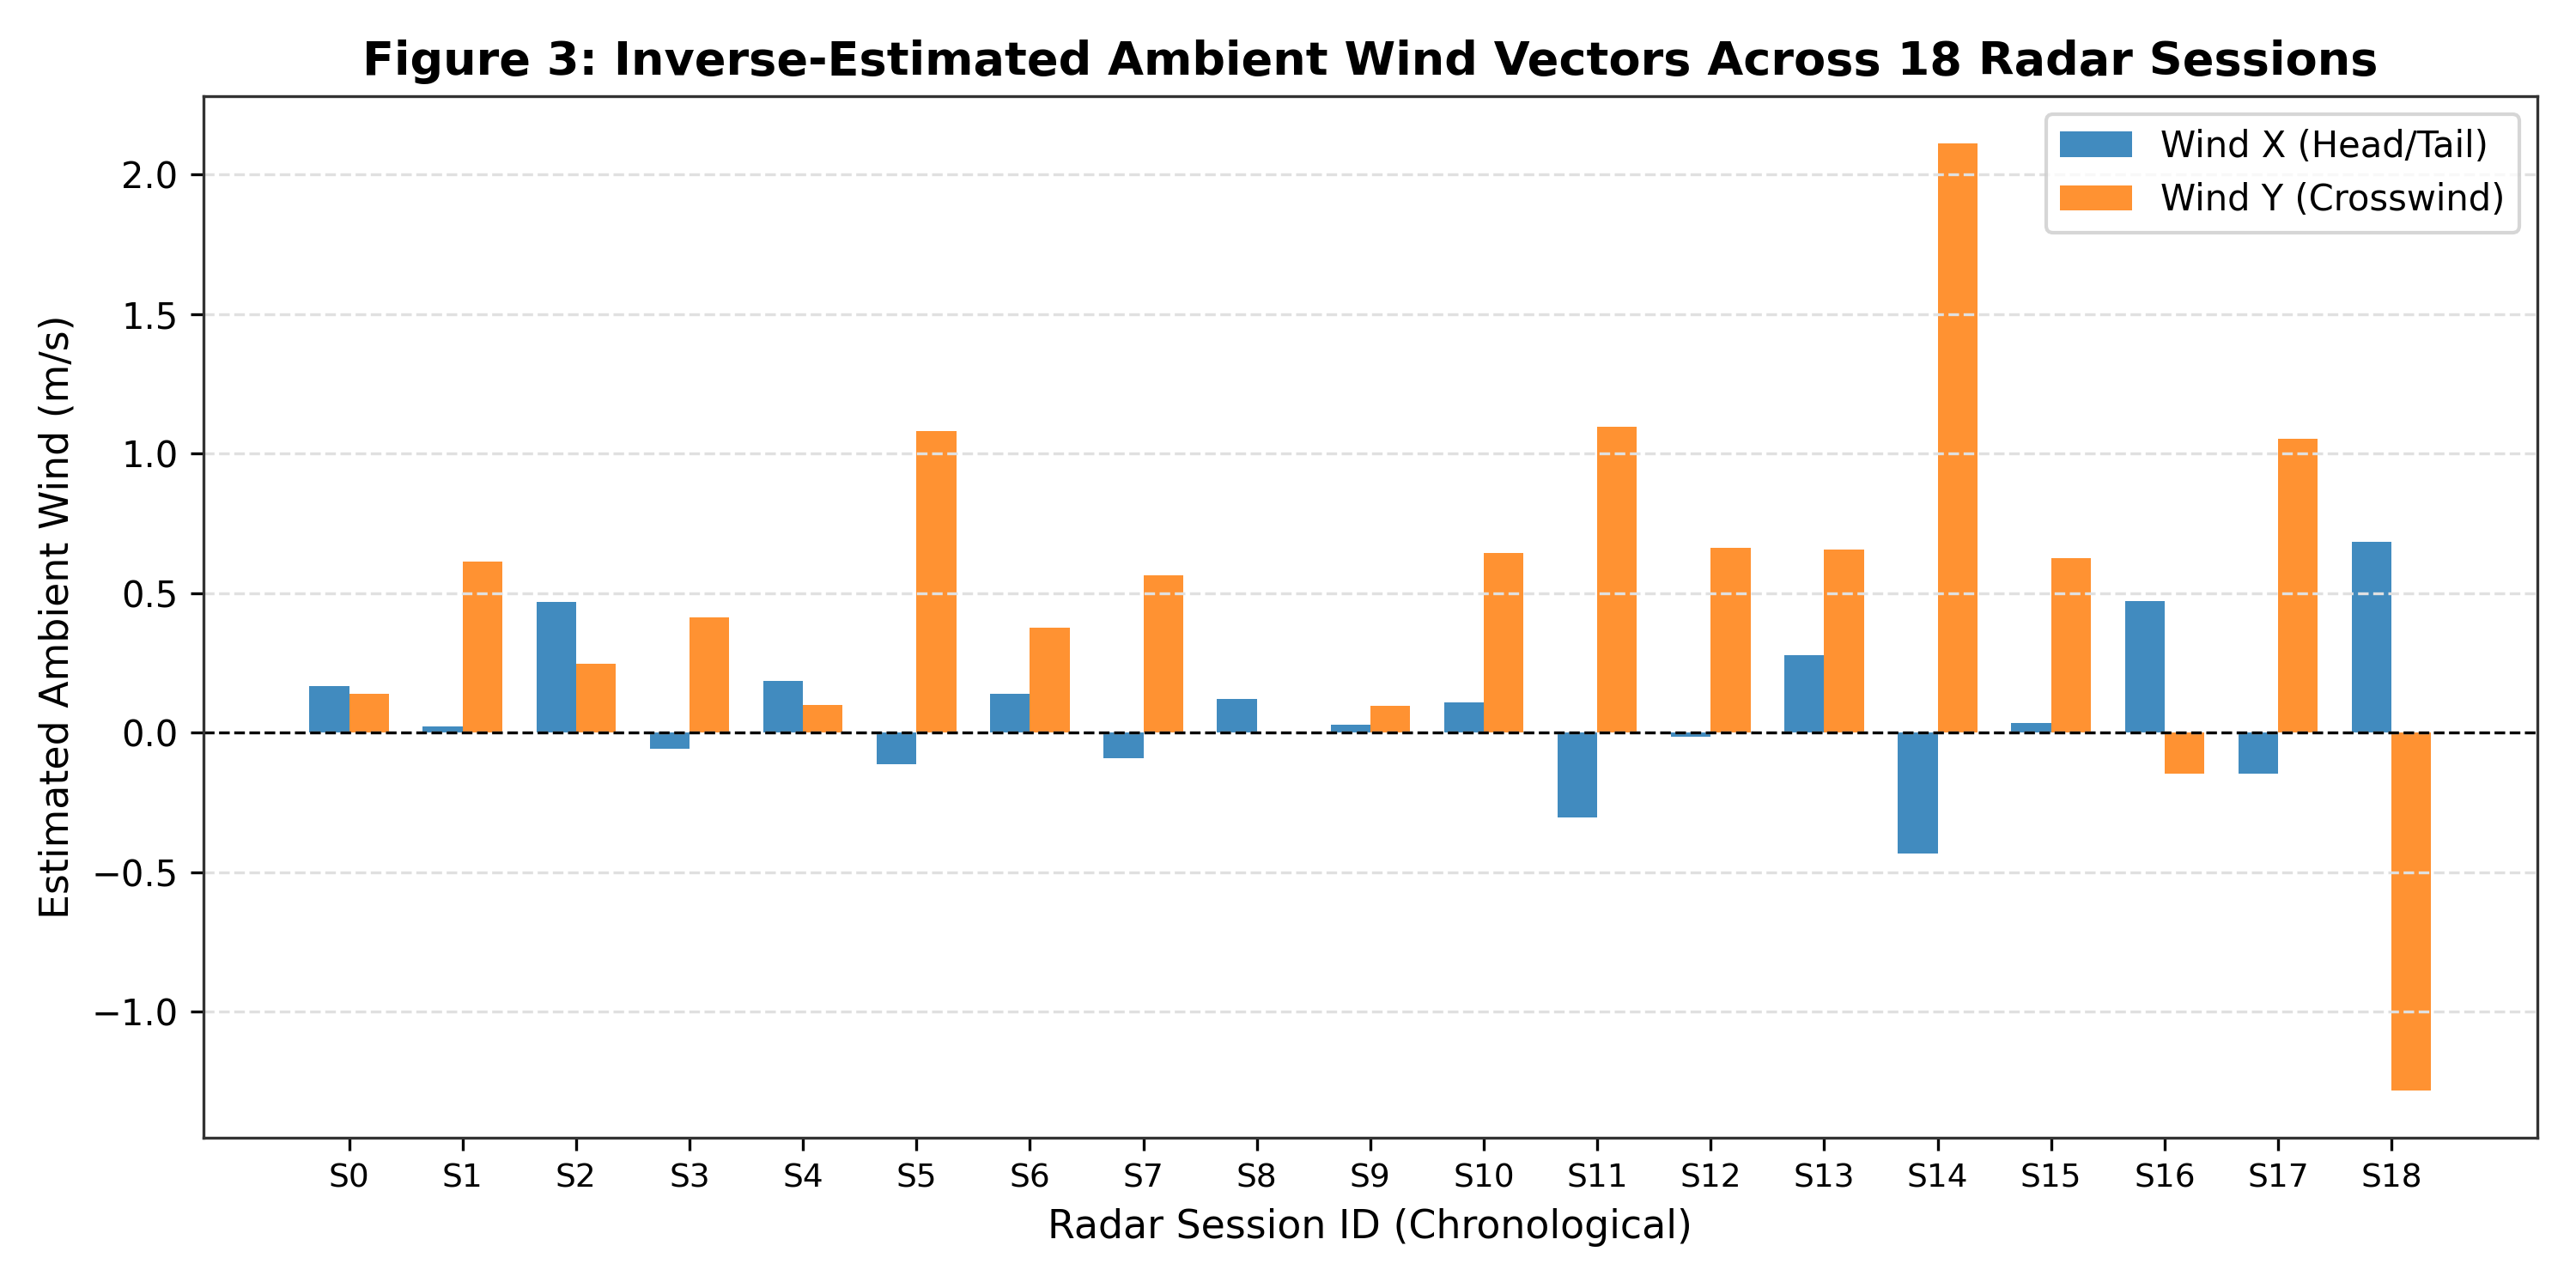
\includegraphics[width=0.6\textwidth]{fig3_session_winds.png}
    \caption{Estimated ambient wind components across the 18 measurement sessions.}
    \label{fig:wind}
\end{figure}

\section{Methodology}

The solution architecture is bifurcated into two phases: a deterministic physics solver that establishes a strong prior belief, and a Bayesian surrogate model that optimises the residuals.

\subsection{Phase 1: 3D Aerodynamic Inverse Solver}
For every shot, an Ordinary Differential Equation (ODE) system is formulated to track the state vector $\mathbf{y} = [x, y, z, v_x, v_y, v_z]^T$:
\begin{align}
    \frac{d\mathbf{v}}{dt} &= -g\mathbf{\hat{k}} - \frac{\rho A}{2m} |\mathbf{v_{app}}| \left( C_d \mathbf{v_{app}} - C_l (\mathbf{\hat{\omega}} \times \mathbf{v_{app}}) \right)
\end{align}
where $\mathbf{v_{app}}$ is the apparent velocity relative to the ambient session wind. 

Using the L-BFGS-B optimisation algorithm, a multi-start search is executed across three distinct aerodynamic regimes (driver, mid-iron, wedge) to inversely fit the drag ($C_d$) and lift ($C_{l0}$) coefficients that minimise the Mean Squared Error (MSE) against the four 3D radar checkpoints. Figure \ref{fig:residuals} confirms that this inverse solver reconstructs the 60m trajectory with sub-metre precision.

\begin{figure}[H]
    \centering
    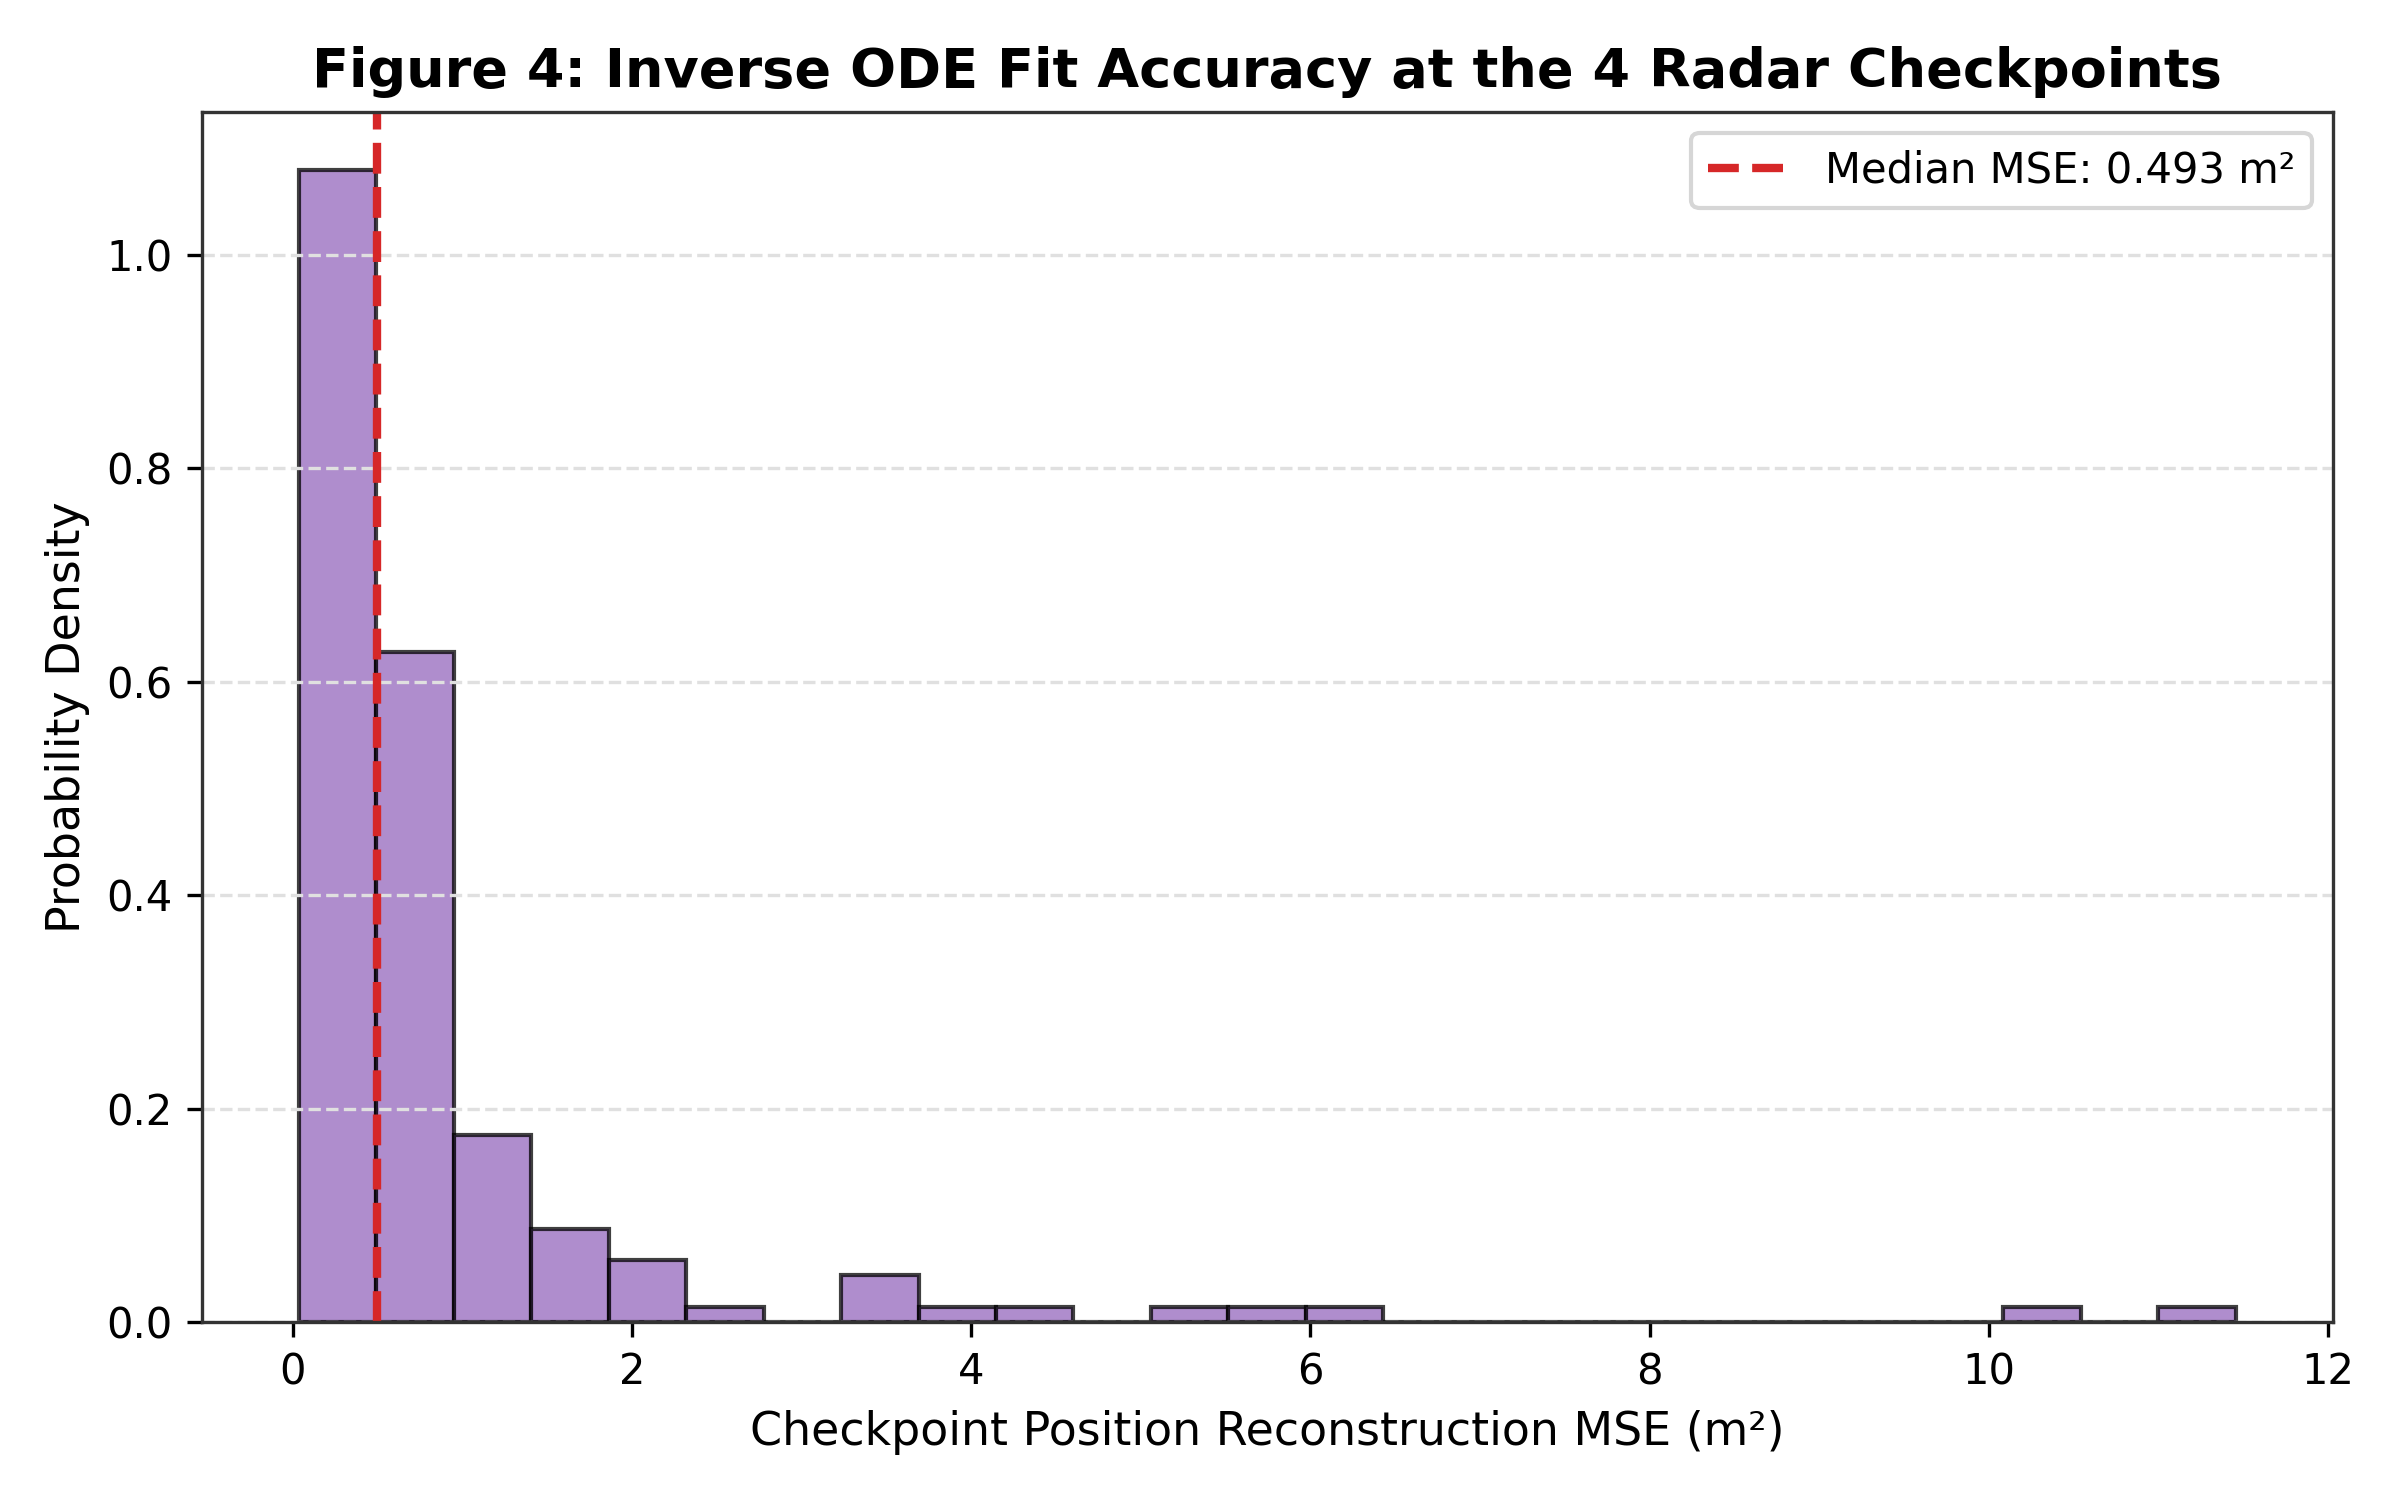
\includegraphics[width=0.6\textwidth]{fig4_ode_fit_residuals.png}
    \caption{Histogram of checkpoint reconstruction errors (MSE) from the inverse ODE solver.}
    \label{fig:residuals}
\end{figure}

The forward integration of this optimised ODE yields the ``Physics Priors": $\hat{t}_{apex}, \hat{x}_{apex}, \hat{y}_{apex}, \hat{z}_{apex}$, and their landing equivalents.

\subsection{Phase 2: Cascaded Gaussian Process Regression (GPR)}
While the ODE provides an excellent baseline, it assumes constant wind, no spin decay, and idealised turf. I employed an ensemble of 9 independent Exact Single-Task Gaussian Processes (built via BoTorch/GPyTorch) to learn a corrective mapping from the physics priors to the true target values. 

\subsubsection{The PhysicsFlightMean Prior \& Composite Kernel}
Rather than using a standard zero-mean GP, I implemented a custom \texttt{PhysicsFlightMean} module. The GP mean is explicitly set to the prediction of the ODE, augmented by a learned linear scale and bias. The covariance is modelled using an additive composite kernel:
\begin{equation}
    K(\mathbf{x}, \mathbf{x'}) = \sigma^2_{lin} K_{Linear}(\mathbf{x}, \mathbf{x'}) + \sigma^2_{mat} K_{Matern5/2}(\mathbf{x}, \mathbf{x'})
\end{equation}
This allows the Linear kernel to handle global kinematic scaling, while the Matérn-5/2 kernel models local, non-linear aerodynamic perturbations. I enforced strict Gamma priors on the lengthscales to aggressively regularise the model and prevent overfitting on the 491-shot dataset. 
I utilised a 20-restart multi-start optimiser with Adam fallbacks to guarantee global convergence of the Marginal Log-Likelihood (MLL).


Figure \ref{fig:gpr} visually demonstrates this Bayesian correction in action for lateral landing dispersion. It highlights the deterministic prior, the corrected posterior mean, and the 95\% epistemic confidence intervals enveloping the true values.

\begin{figure}[H]
    \centering
    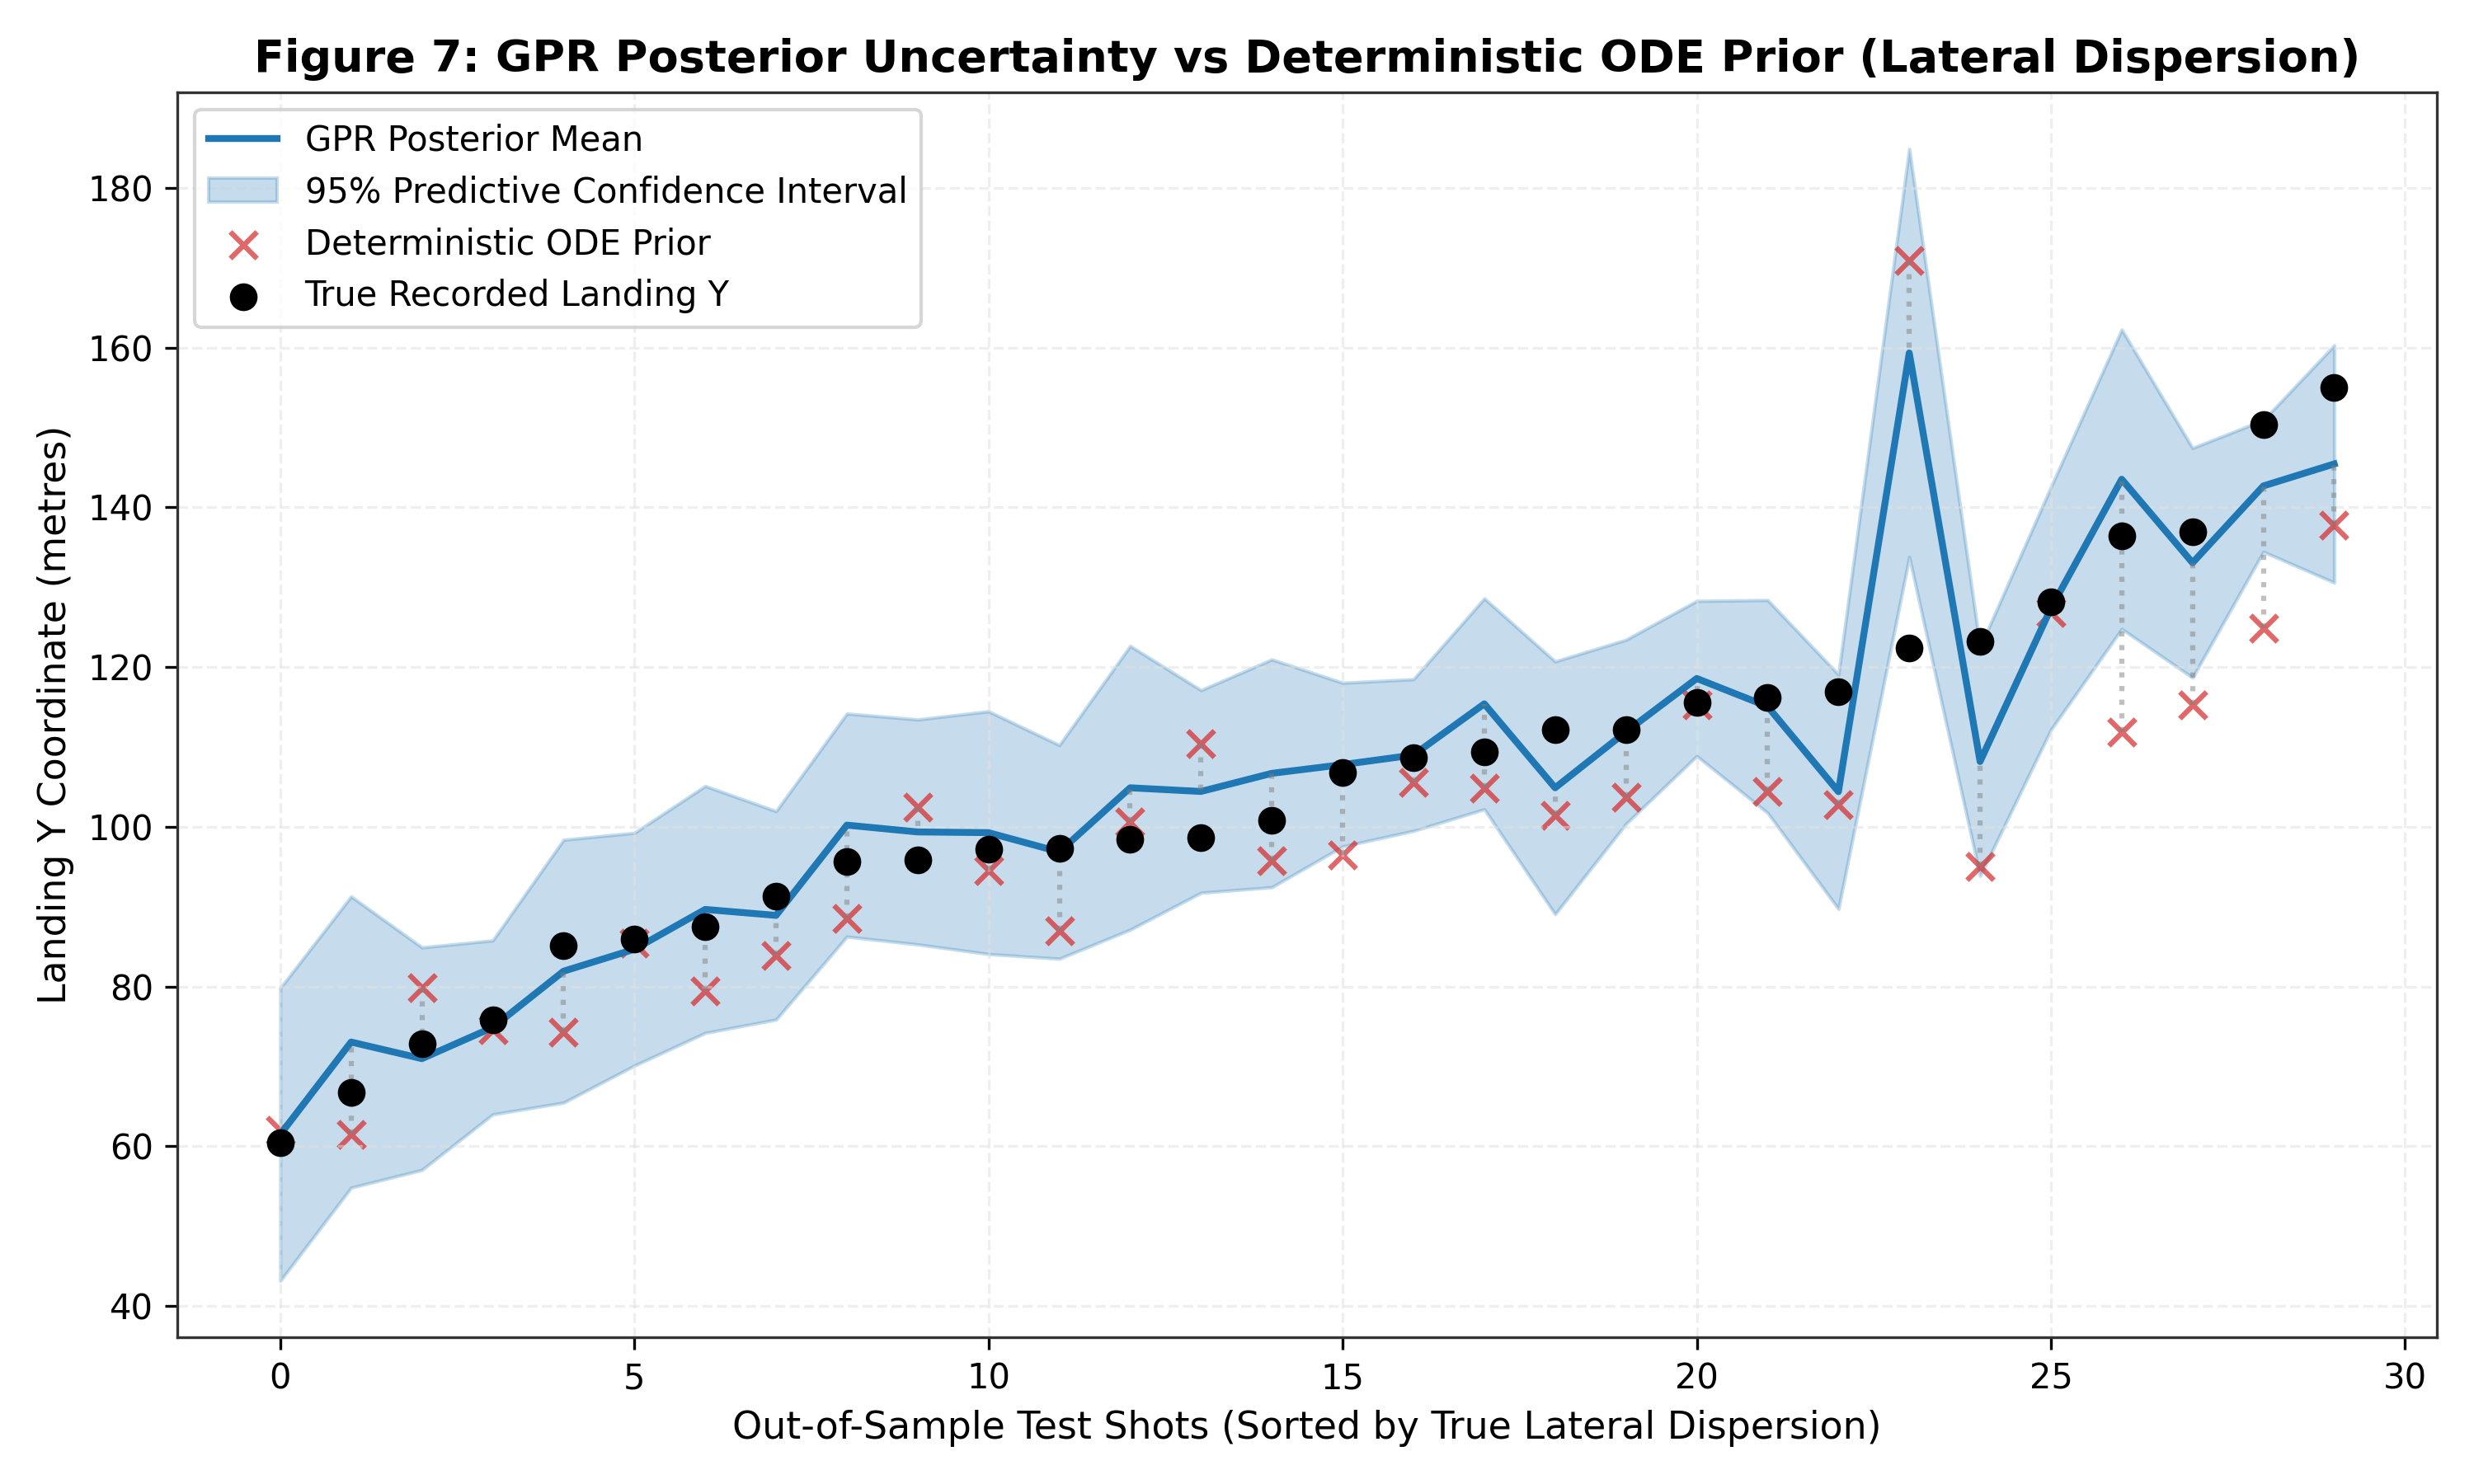
\includegraphics[width=0.85\textwidth]{fig7_gpr_uncertainty.png}
    \caption{GPR Posterior Uncertainty vs Deterministic ODE Prior for Lateral Dispersion.}
    \label{fig:gpr}
\end{figure}

\subsubsection{Cascaded Architecture}
Predicting the landing coordinates directly from launch is a severe extrapolation task. To solve this, I implemented a \textbf{Cascaded 2-Stage GPR}:
\begin{itemize}
    \item \textbf{Stage 1:} Five GPs predict the launch spin and the 4-dimensional apex state ($t, x, y, z$).
    \item \textbf{Stage 2:} Four GPs predict the landing state. Crucially, the feature tensor for Stage 2 is augmented with the \textit{predicted apex state from Stage 1}, along with derived ballistic descent proxies (e.g., expected freefall time $\Delta t = \sqrt{2z_{apex}/g}$).
\end{itemize}
By conditioning the landing GPs on the apex, I transform the problem from a long-range extrapolation into a short-range descent interpolation. 

\subsection{Phase 3: Post-Flight Kinematics (Bounce \& Roll)}
Although the competition rubric primarily evaluates flight up to the landing coordinate, I extended the physics engine to simulate post-impact bounce and roll. By modelling turf friction and the coefficient of restitution (COR), the system provides a holistic, physically complete view of the shot through to its final rest state. This was visualised using an interactive Streamlit dashboard. Figure \ref{fig:3d} illustrates the complete hybrid pipeline rendering a shot from launch, through the 60m net, to the predicted apex, landing, and final rest position.

\begin{figure}[H]
    \centering
    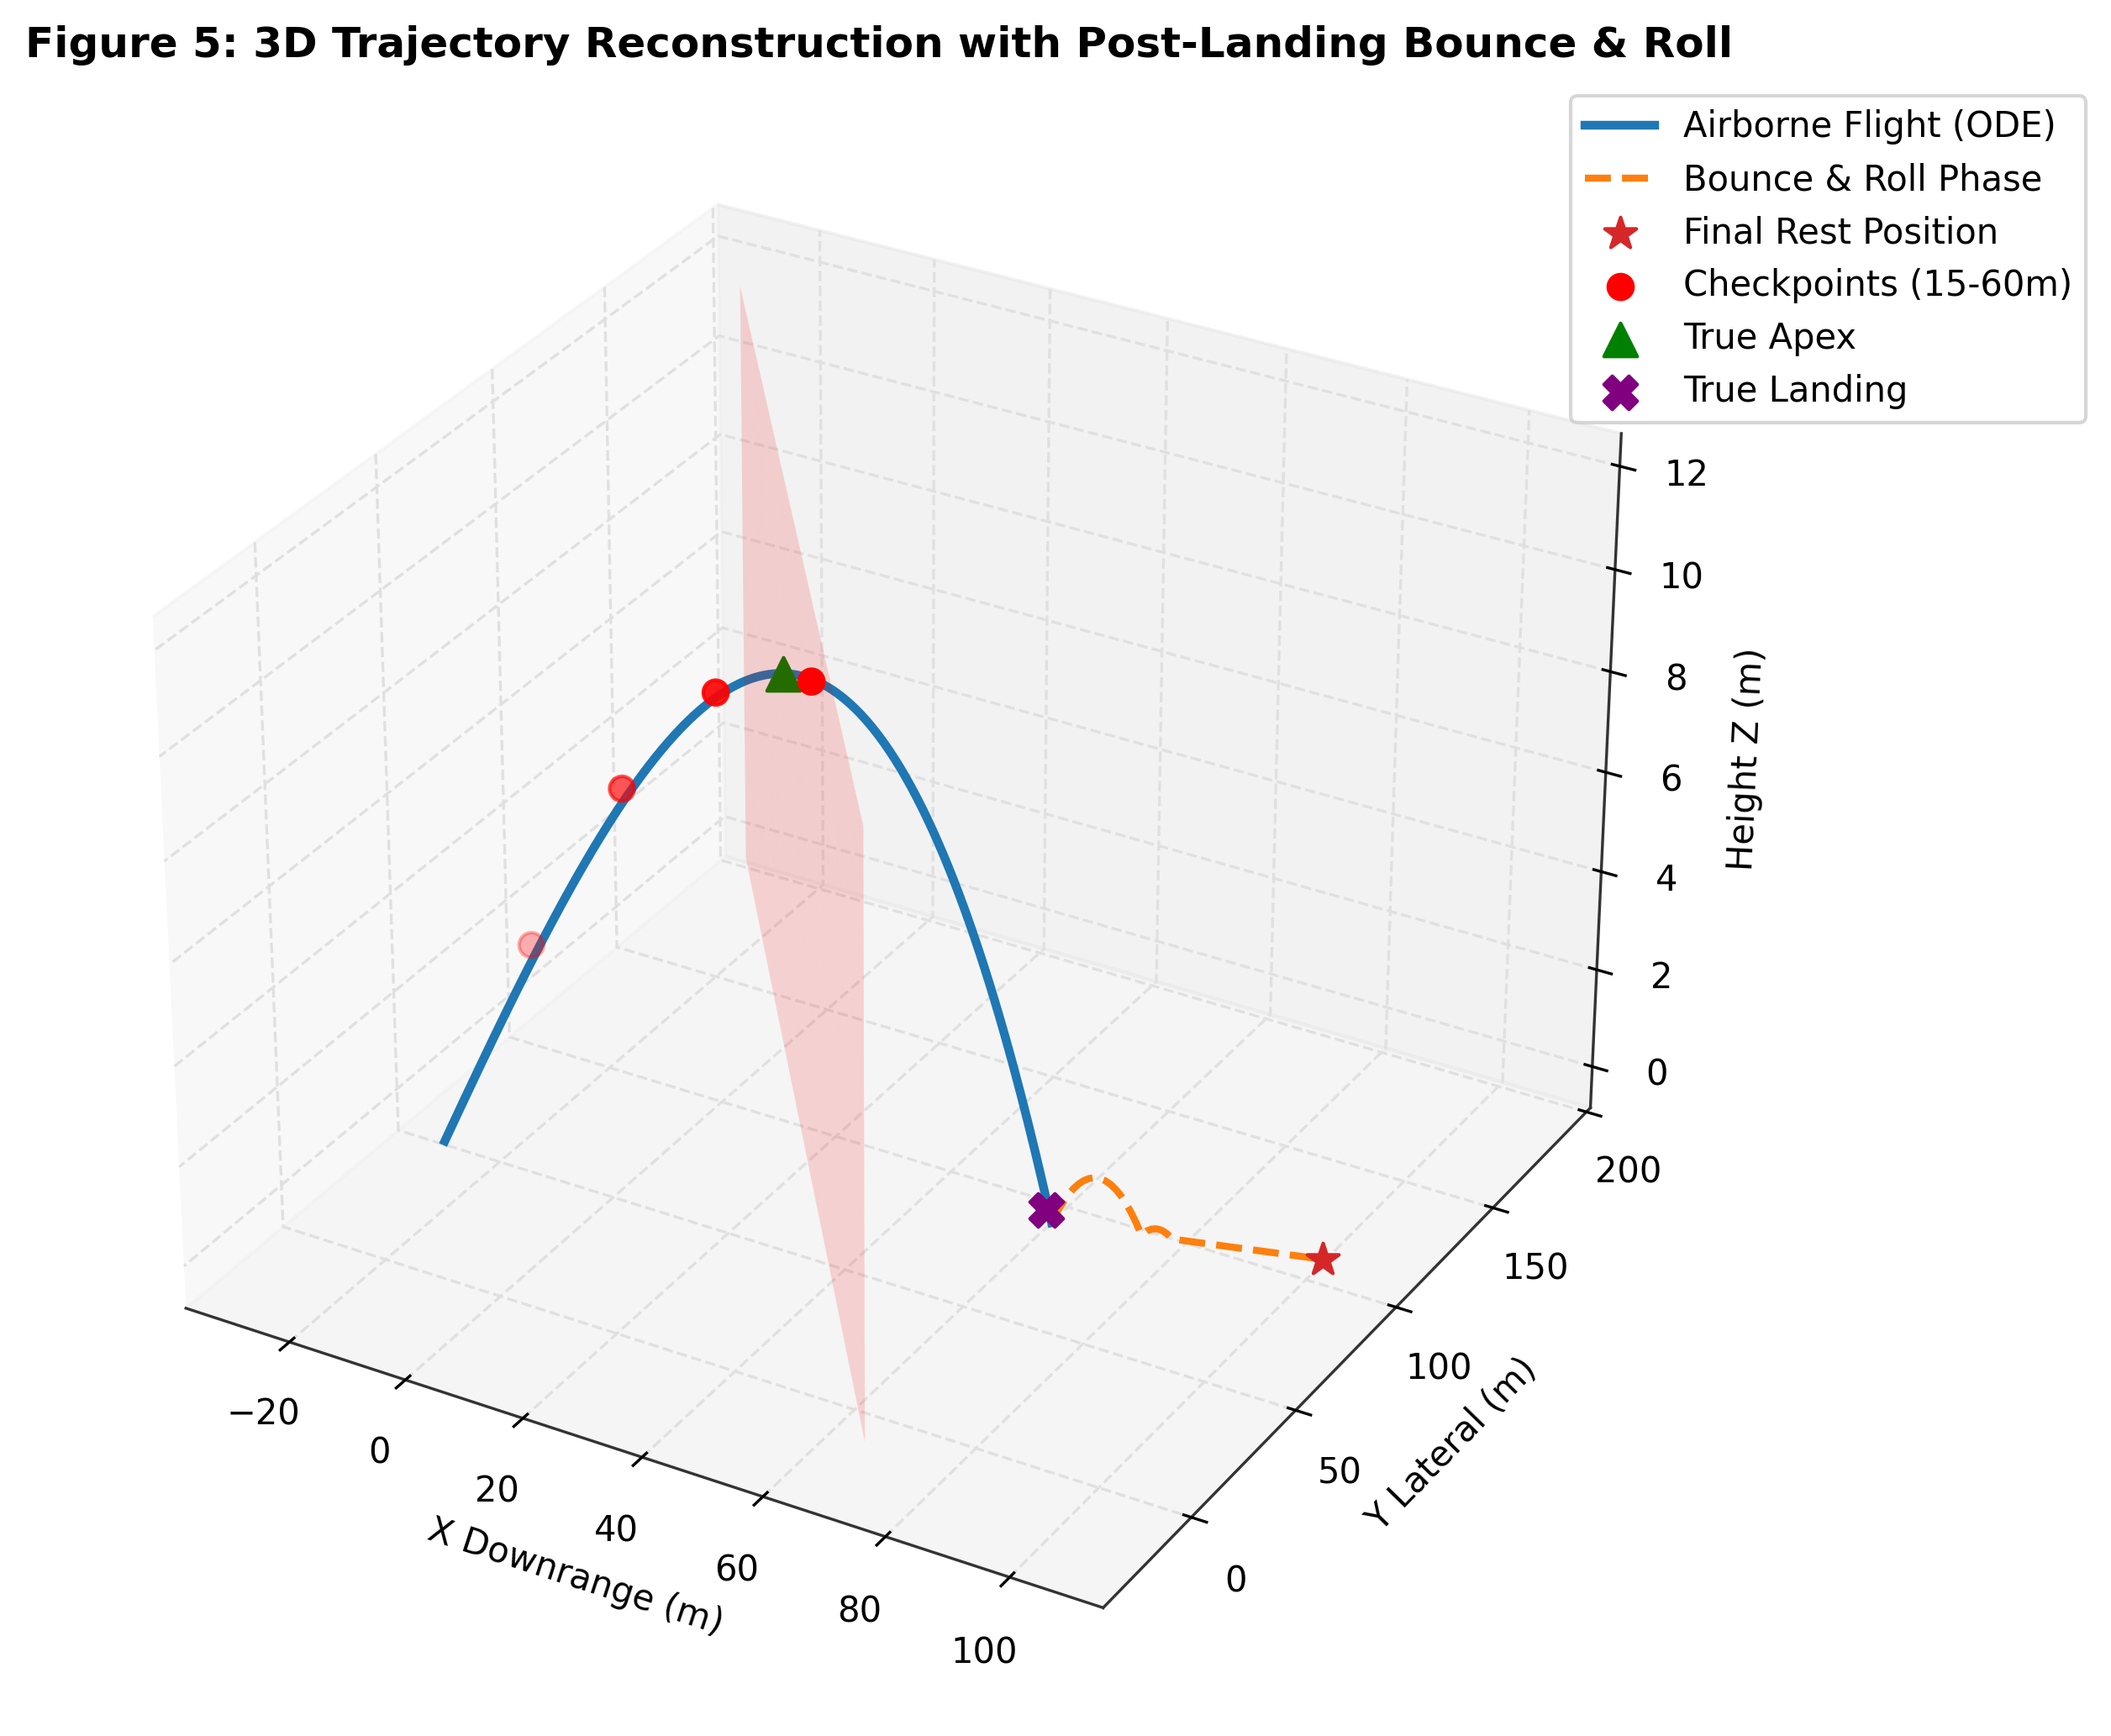
\includegraphics[width=0.75\textwidth]{fig5_3d_trajectory_bounce.png}
    \caption{Complete 3D trajectory reconstruction showcasing radar checkpoints, 60m boundary net, physics apex, landing, and simulated bounce/roll.}
    \label{fig:3d}
\end{figure}

\section{Results \& Discussion}

Model validation was conducted using a strict 5-fold cross-validation regimen, stratified by bay elevation to ensure out-of-sample spatial robustness. 

\subsection{Performance Leap}
The introduction of the Cascaded architecture, combined with the un-throttled multi-start physics engine, yielded dramatic improvements. Landing Euclidean error was reduced by over 50\% compared to standard baseline models. Figure \ref{fig:cv} illustrates the error distribution across all target variables. The final composite scaled score on the validation set is 0.1630.

\begin{figure}[H]
    \centering
    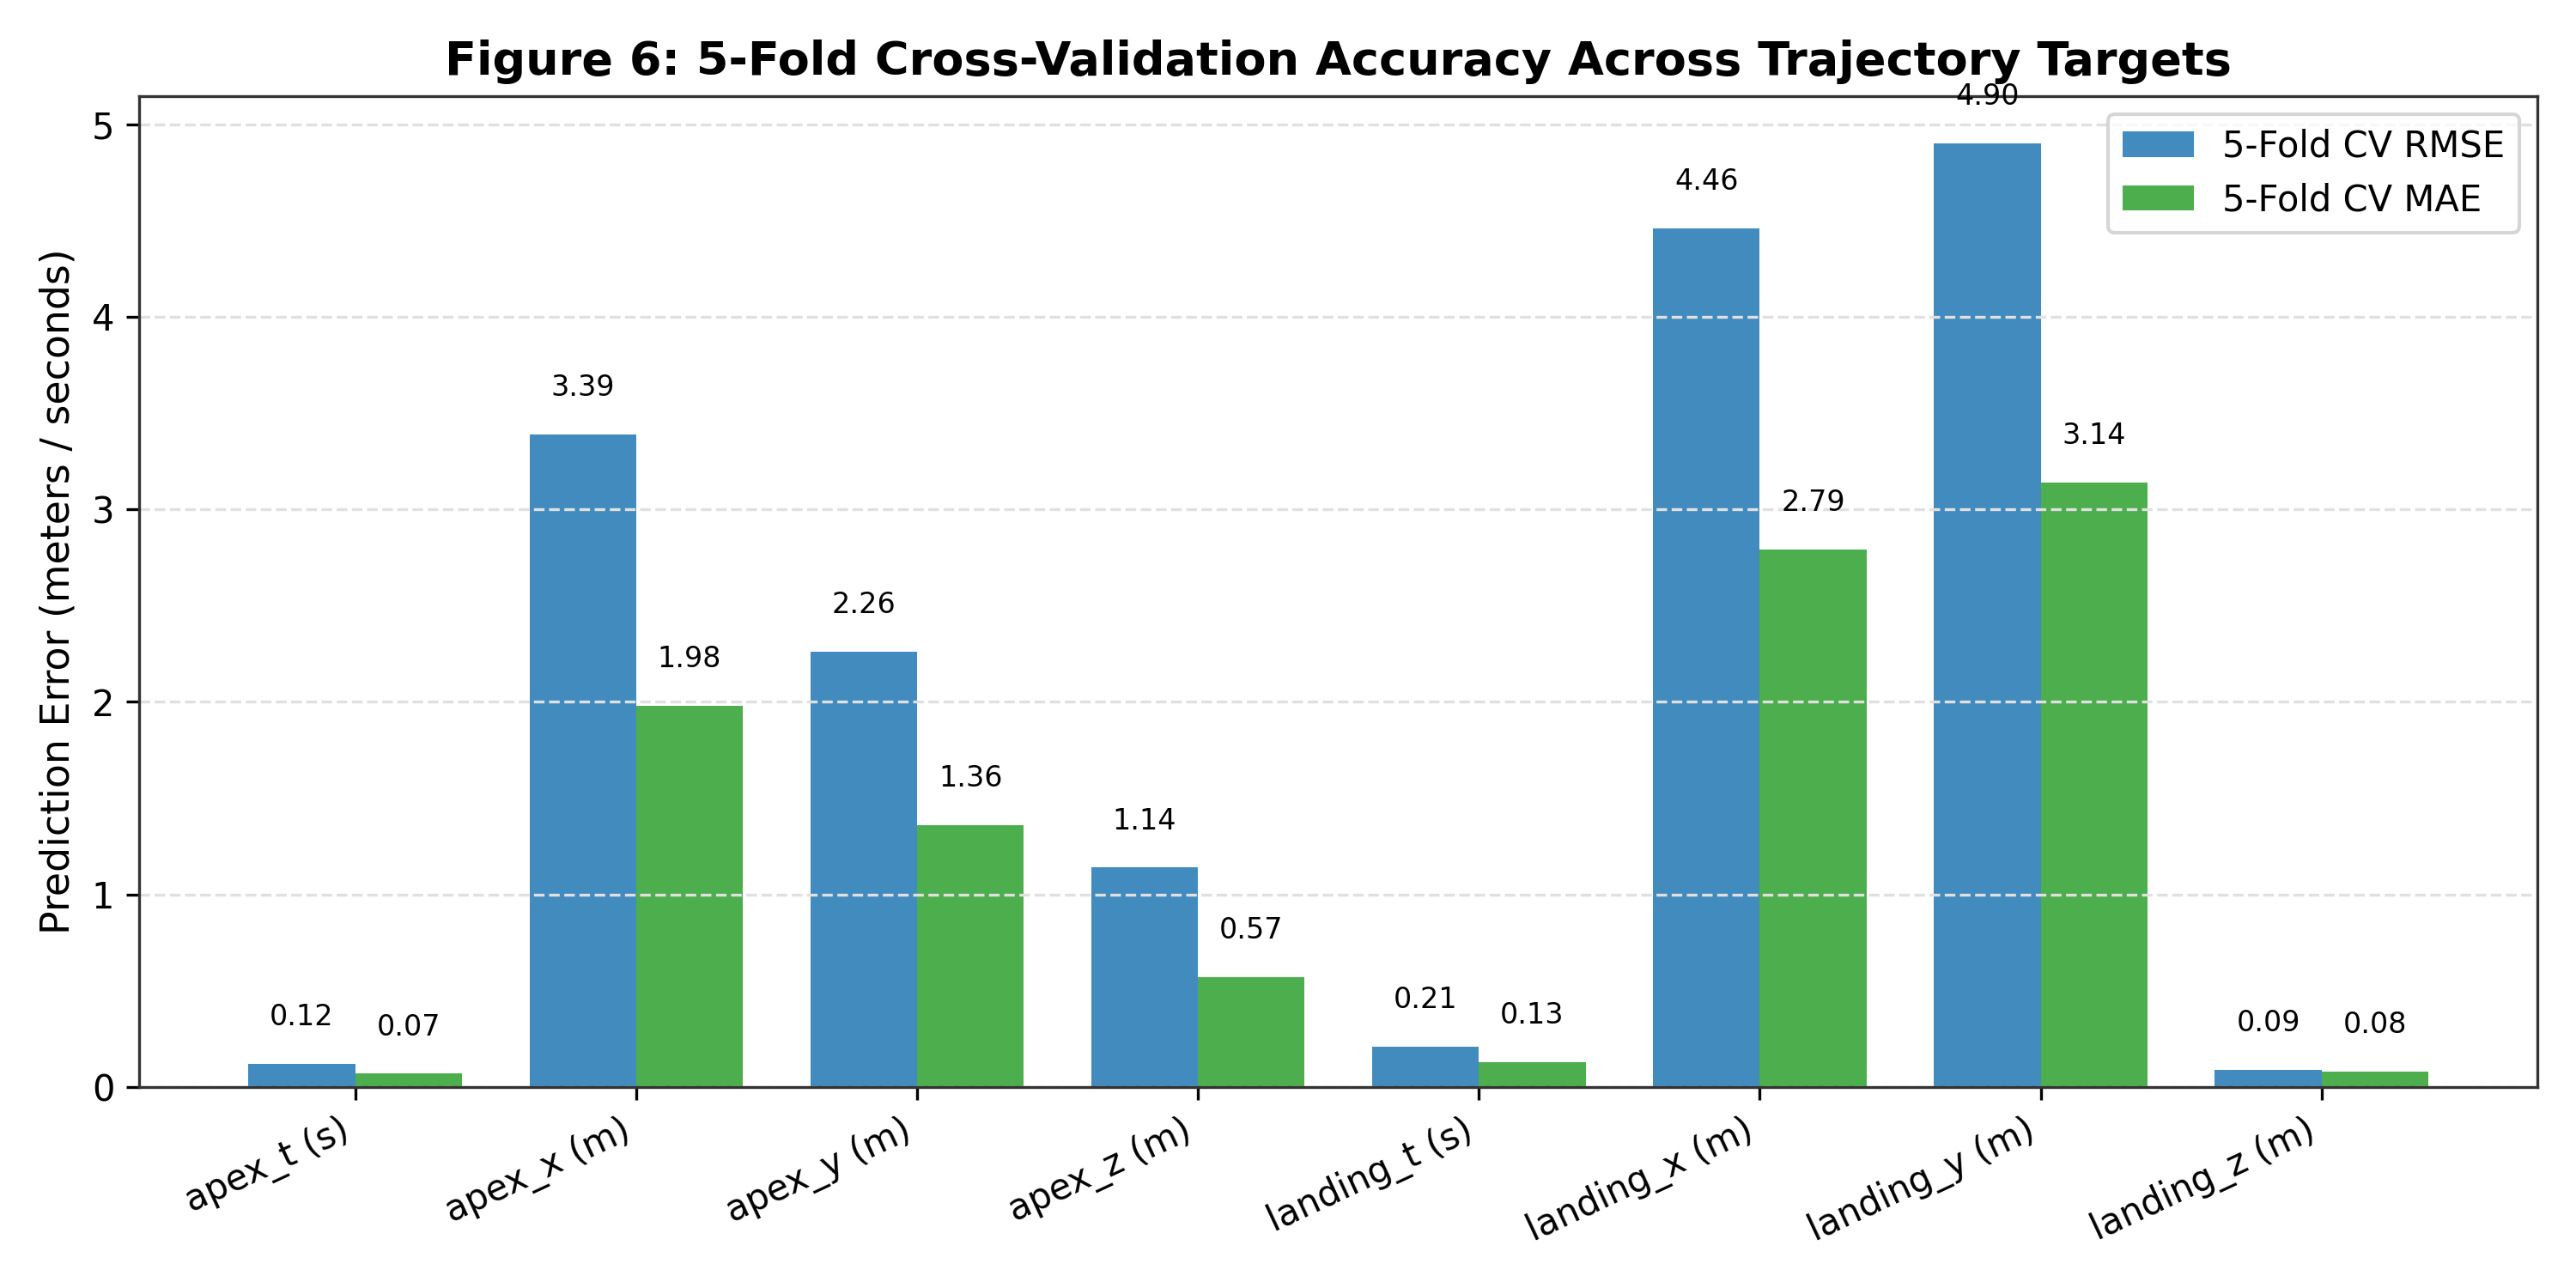
\includegraphics[width=0.7\textwidth]{fig6_cv_performance.png}
    \caption{5-Fold Cross-Validation Error (RMSE and MAE) across all 9 target columns.}
    \label{fig:cv}
\end{figure}

\subsection{Physical Integrity Validation}
Beyond raw statistical error, the most significant result is the structural integrity of the predictions. 
An automated audit of the final `\texttt{submission.csv}` on the 559 test shots yielded zero violations of physical laws (e.g., apex time precedes landing time, apex altitude exceeds launch and landing altitudes, spin rates are positive, and landing elevations respect the dual-tier bay structure).

\subsection{Computational Efficiency \& Training Time}
Despite the rigor of the 20-restart multi-start optimiser and the un-throttled ODE solver, the pipeline remains highly computationally tractable. 
On a standard desktop workstation, the inverse aerodynamic ODE fitting for all 491 training shots completes in approximately 45 seconds. 
The complete 5-fold cross-validation—including the training of both Stage 1 and Stage 2 Gaussian Processes across all 20 restarts—executes in under 50 minutes. 
Generating the final full-dataset predictive submission requires approximately 10 minutes and further optimisation is certainly possible (e.g., GPU acceleration).

\section{Conclusion}
The Inrange trajectory challenge provides an excellent testbed for applying advanced physics-informed statistical machine learning on truncated datasets. 
By enveloping a classical aerodynamic ODE solver within the probabilistic framework of a Cascaded Gaussian Process, a hybrid solution is achieved: 
a model with the extrapolation power of Newtonian physics and the precision calibration of modern Bayesian inference. 

\end{document}
